%! TEX root = **/000-main.tex
% vim: spell spelllang=en:
\chapter{Discussion of results}
\label{sec:analysis}

% TODO: no em convenc el titol
\section{Paired t-test results}

Although the previous results are interesting, they are not conclusive and
are based merely on the visual inspection of the plots. In order to draw
conclusions, we need to perform a statistical test to see if there is
really any meaningful difference between the models.

As explained in \cref{sec:paired-t-test}, we will use the 5\texttimes2
paired $t$-test. With this test, the null hypothesis is that the two models
have equal performance.

\subsection{RBF vs Arc-sine}

We start by comparing the RBF kernel with the normalized arc-sine kernel for
different values of $\sigma_w$ and $\gamma$ using $nRMSE$ as the performance
measure. The results are shown in \cref{fig:paired-ttest-rbf-asinnorm},
which shows the matrix of $p$-values shaded by the significance level,
darker the color, the more significant the difference between the two models.

% TODO: is this the most sensible way or should we approach it differently?
The values of $\epsilon$ and $C$ are selected as the ones which obtained
the performed best for each $\sigma$ and $\gamma$.

\begin{figure}[H]
    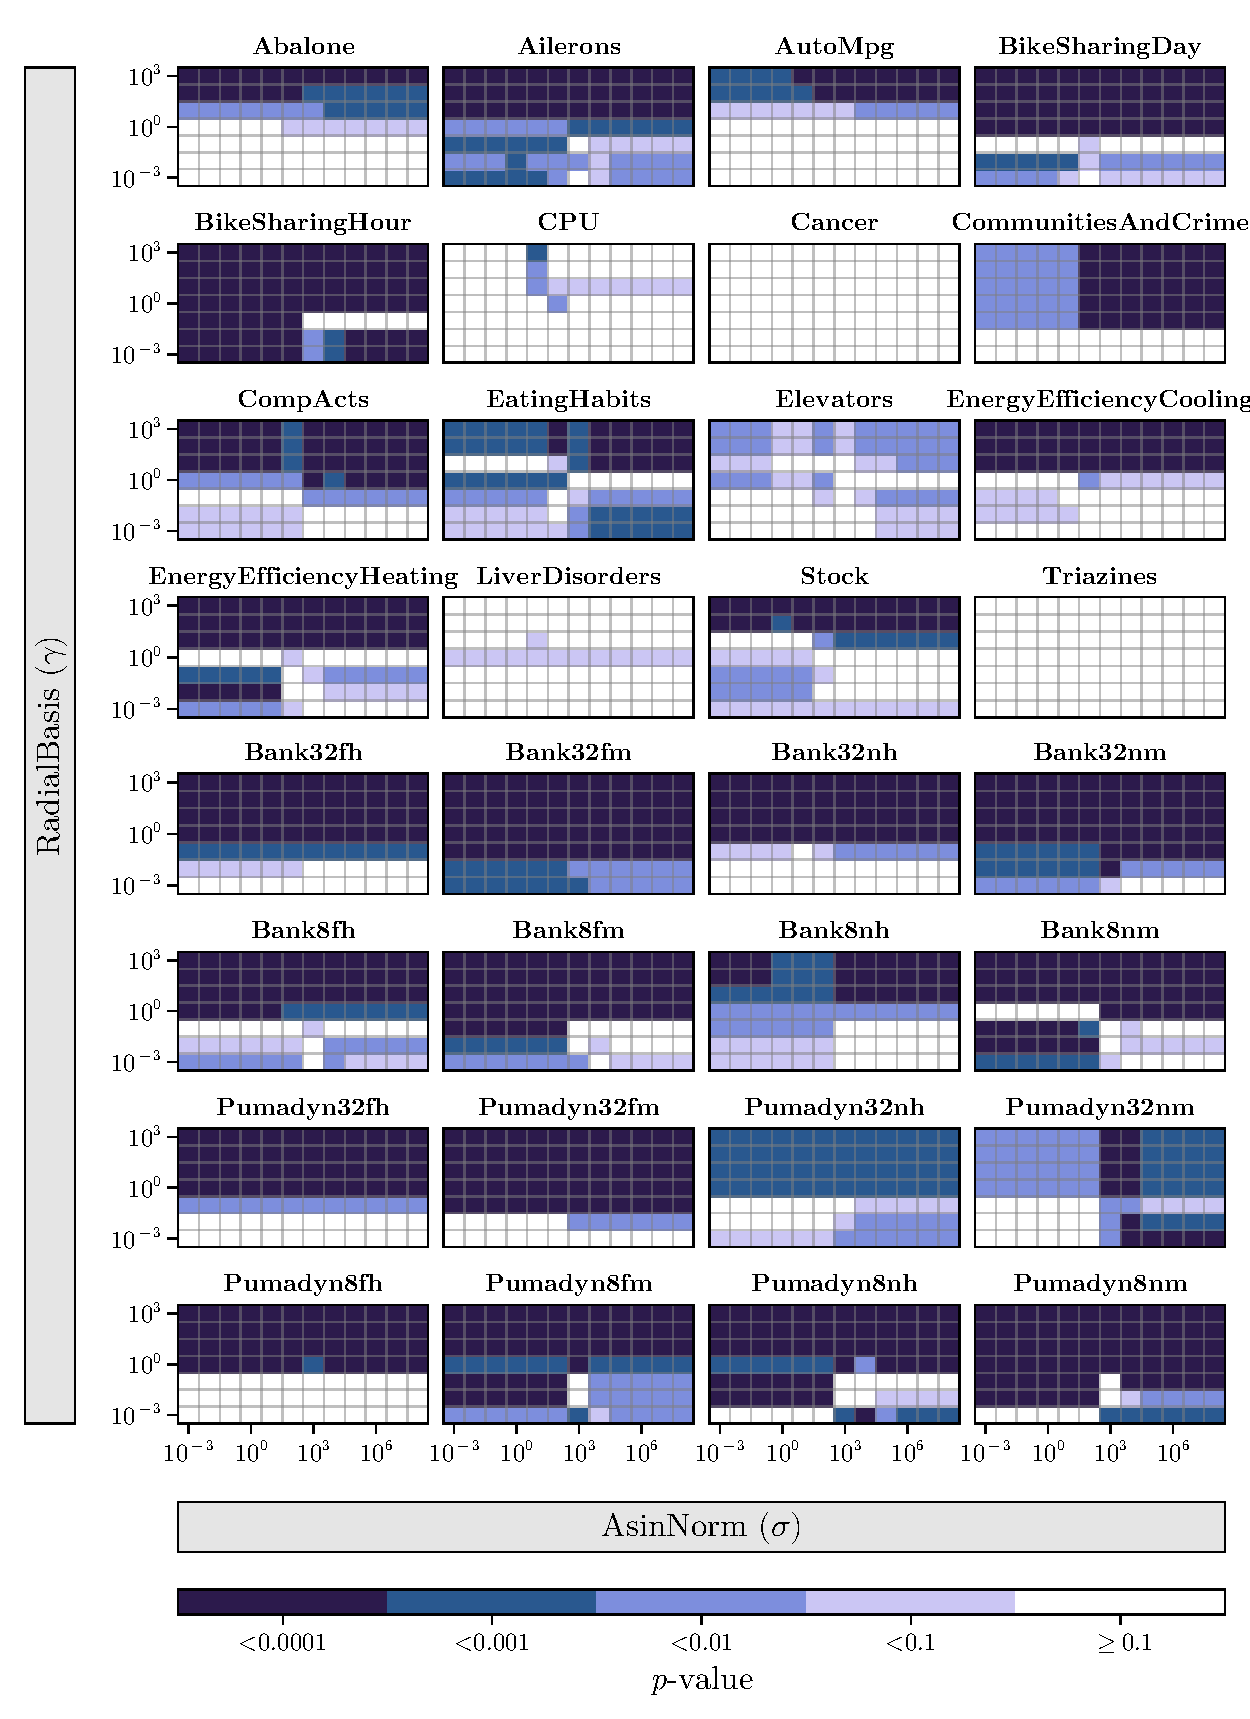
\includegraphics[width=0.9\textwidth]{plots/heatmaps_rbf_asinnorm_pvalues}
    \caption{p values}
    \label{fig:paired-ttest-rbf-asinnorm}
\end{figure}

In \cref{fig:paired-ttest-rbf-asinnorm}, we can see that for datasets
\texttt{Cancer} and \texttt{Triazines}, there is no pair of hyperparameter
values for which the difference between the two models is significant even at
$\alpha=0.1$. For \texttt{LiverDisorders} and \texttt{Elevators}, the significance
level is not below $\alpha=0.01$ for any pair of hyperparameters.

The matrices shown in \cref{fig:paired-ttest-rbf-asinnorm} show which are the
pairs which are statistically different, but do not show the magnitude or
direction of the difference. For that, we can take the mean values of
the difference in $NRMSE$ between the two models for each pair of hyperparameters
and plot them as shown in \cref{fig:paired-ttest-rbf-asinnorm-diff}.

The plot illustrates the difference between the RBF and normalized arc-sine
kernels. Positive values indicate that the RBF had a higher $NRMSE$ than the
normalized arc-sine kernel. Results that had a $p$-value higher than $\alpha=0.001$
have been removed (white cells).

%  TODO: add pattern or something so the color can be seen in b/w
\begin{figure}[H]
    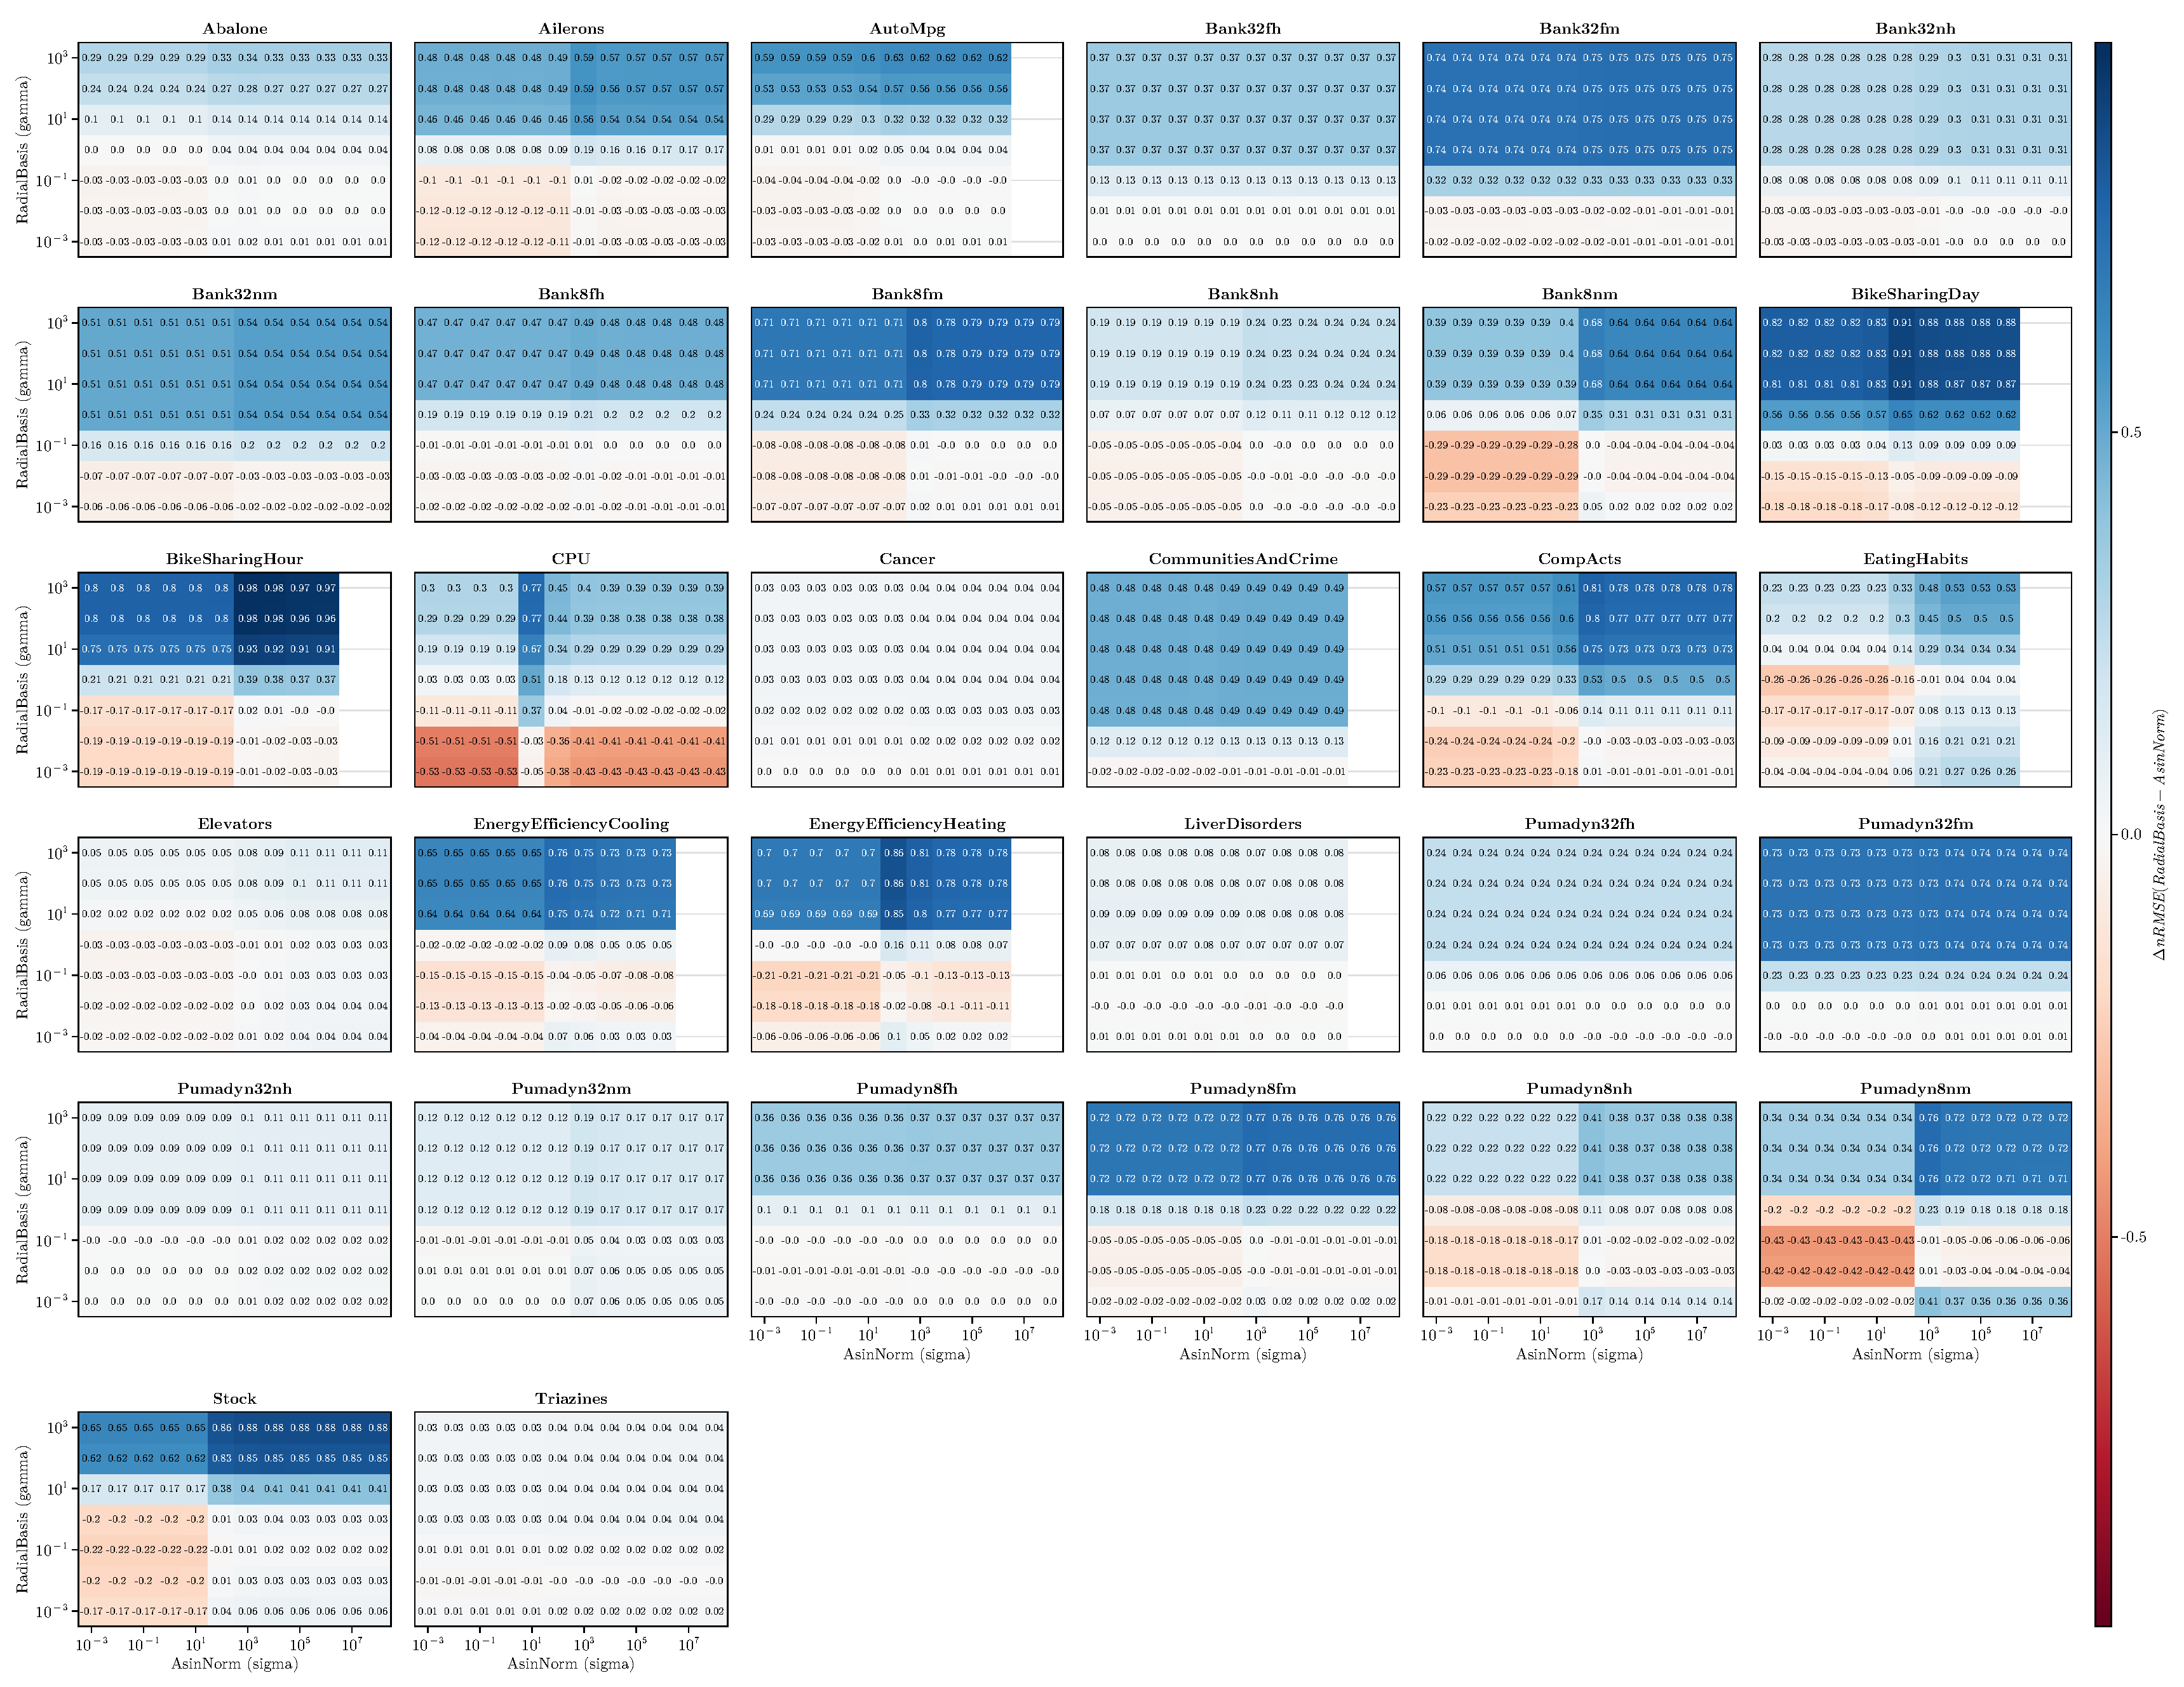
\includegraphics[width=0.9\textwidth]{plots/heatmaps_rbf_asinnorm}
    \caption{Difference between nRMSE of RBF and normalized arc-sine kernels ($\alpha=0.001$)}
    \label{fig:paired-ttest-rbf-asinnorm-diff}
\end{figure}

% \Cref{fig:heatmaps-rbf-asinnorm} shows the difference between the nRMSE of the
% RBF and the normalized arc-sine kernel.
%
% Positive values (in blue) indicate that for that
% combination of $\sigma_w$ and $\gamma$, the normalized arc-sine kernel
% outperforms the RBF kernel.
% Negative values (in red) indicate that the RBF
% kernel performs better than the normalized arc-sine kernel.
% The darker the color, the bigger the difference.
%
% We can observe 3 different behaviours:
% \begin{itemize}
%     \item The difference between the RBF and normalized arc-sine
%           kernels is barely noticeable: \texttt{Cancer}, \texttt{LiverDisorders},
%           \texttt{Triazines}, \dots. Looking at the results from the previous
%           sections, these are \emph{hard} datasets, in the sense that the
%           \emph{nRMSE} obtained by both the RBF and other kernels is high (>0.8).
%
%     \item There is no clear effect of $\sigma_w$ on the
%           performance of the normalized arc-sine kernel: \texttt{Bank32fh},
%           \texttt{Bank32fm}, \texttt{CommunitiesAndCrime}, \texttt{Pumadyn32fm}, \dots
%
%     \item There is threshold for $\sigma_w$ where the normalized
%           arc-sine kernel goes from performing worse than the RBF kernel to
%           performing equally or better than RBF.
% \end{itemize}
%
% % TODO: explain better
% Again, the \texttt{CPU} dataset exhibits a different behaviour where for
% $\sigma_w=0.1$ it is able to match the performance of the RBF kernel, but
% all the others it's significantly worse.
%
% \begin{figure}[H]
%     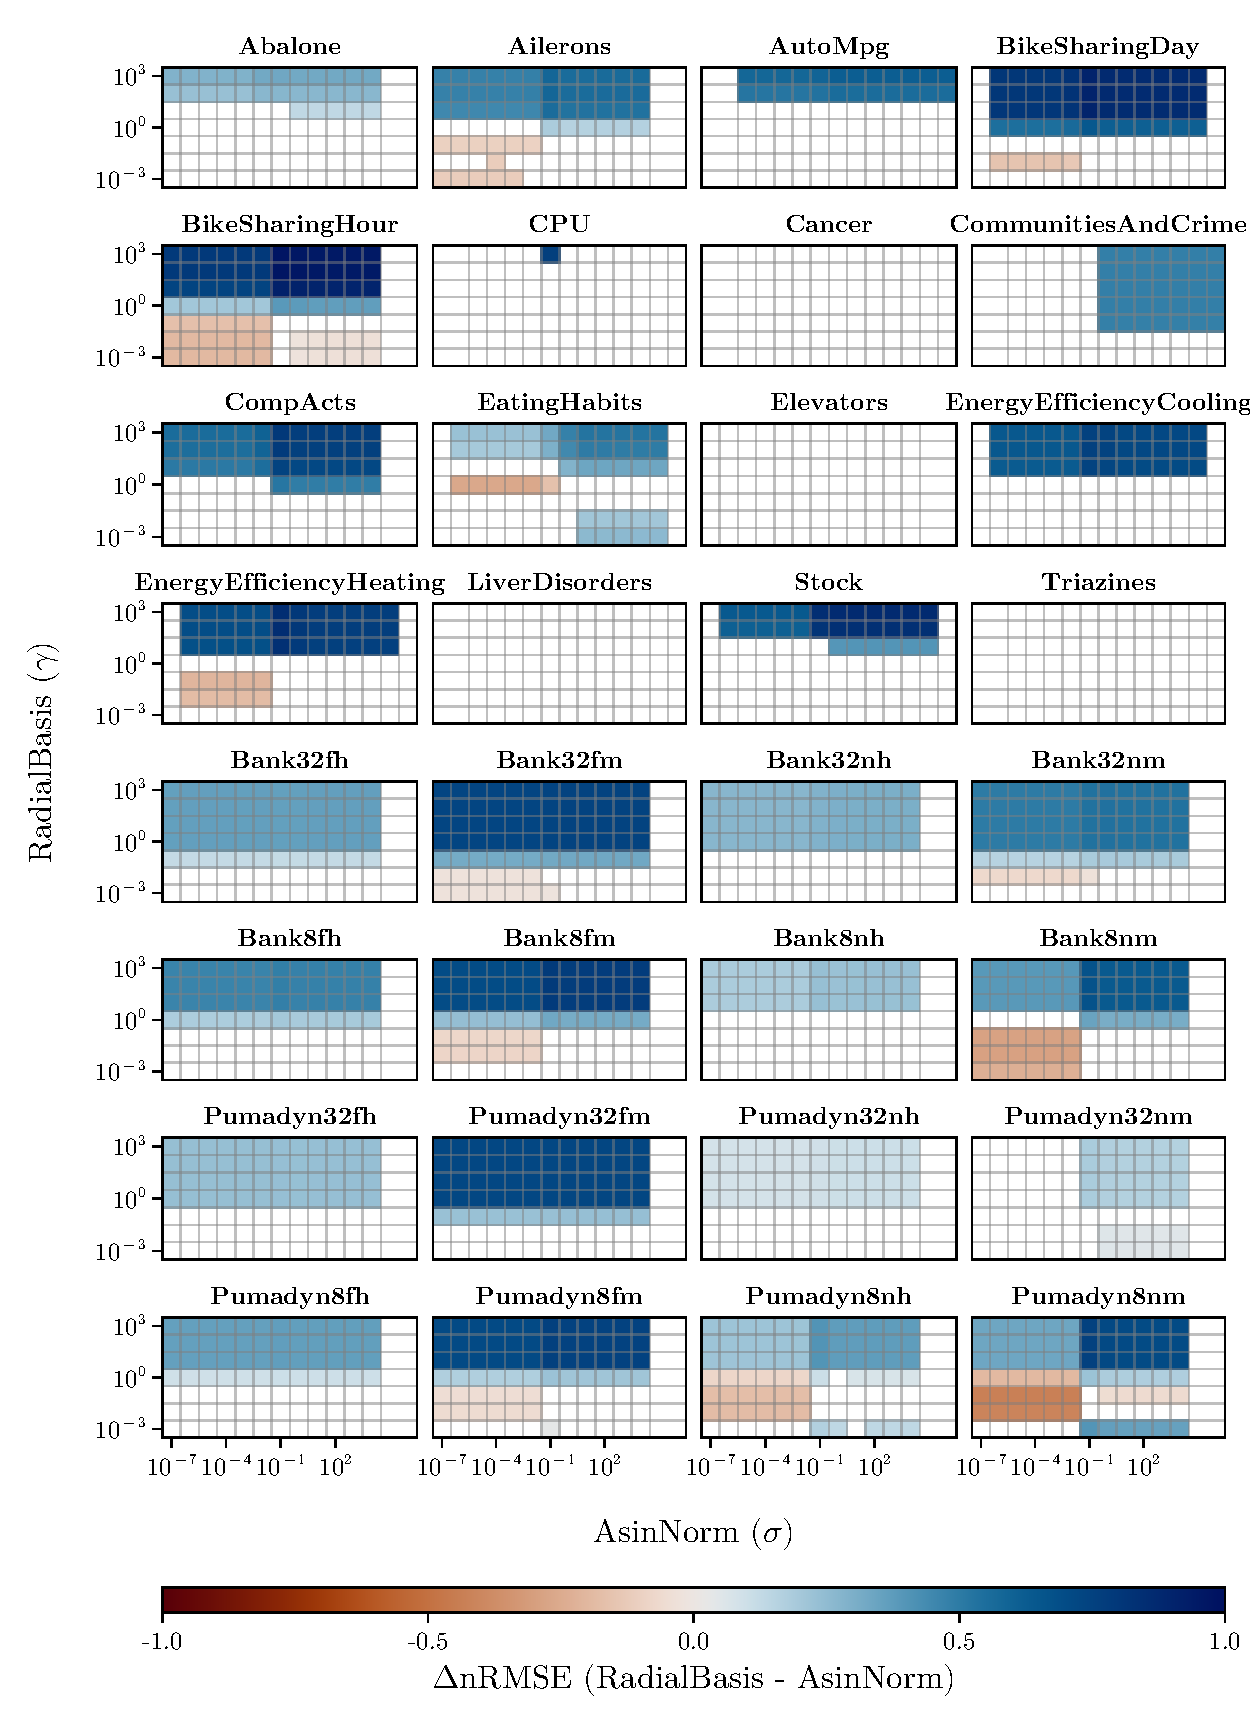
\includegraphics[width=0.9\textwidth]{plots/heatmaps_rbf_asinnorm_s}
%     \caption{Difference between nRMSE of RBF and normalized arc-sine kernels}
%     \label{fig:heatmaps-rbf-asinnorm}
% \end{figure}

\subsection{Arc-sine vs normalized arc-sine}

\Cref{fig:heatmaps-asin-asinnorm} shows the $p$-values for the difference between
the non normalized and the normalized arc-sine kernels. All datasets seem to have
a region on the top right corner where the difference is not very significant.
We can conjecture that for values of $\sigma$ big enough, the normalized and
non-normalized arc-sine kernels perform similarly. The only notable exception is
\texttt{BikeSharingHour}.

\begin{figure}[H]
    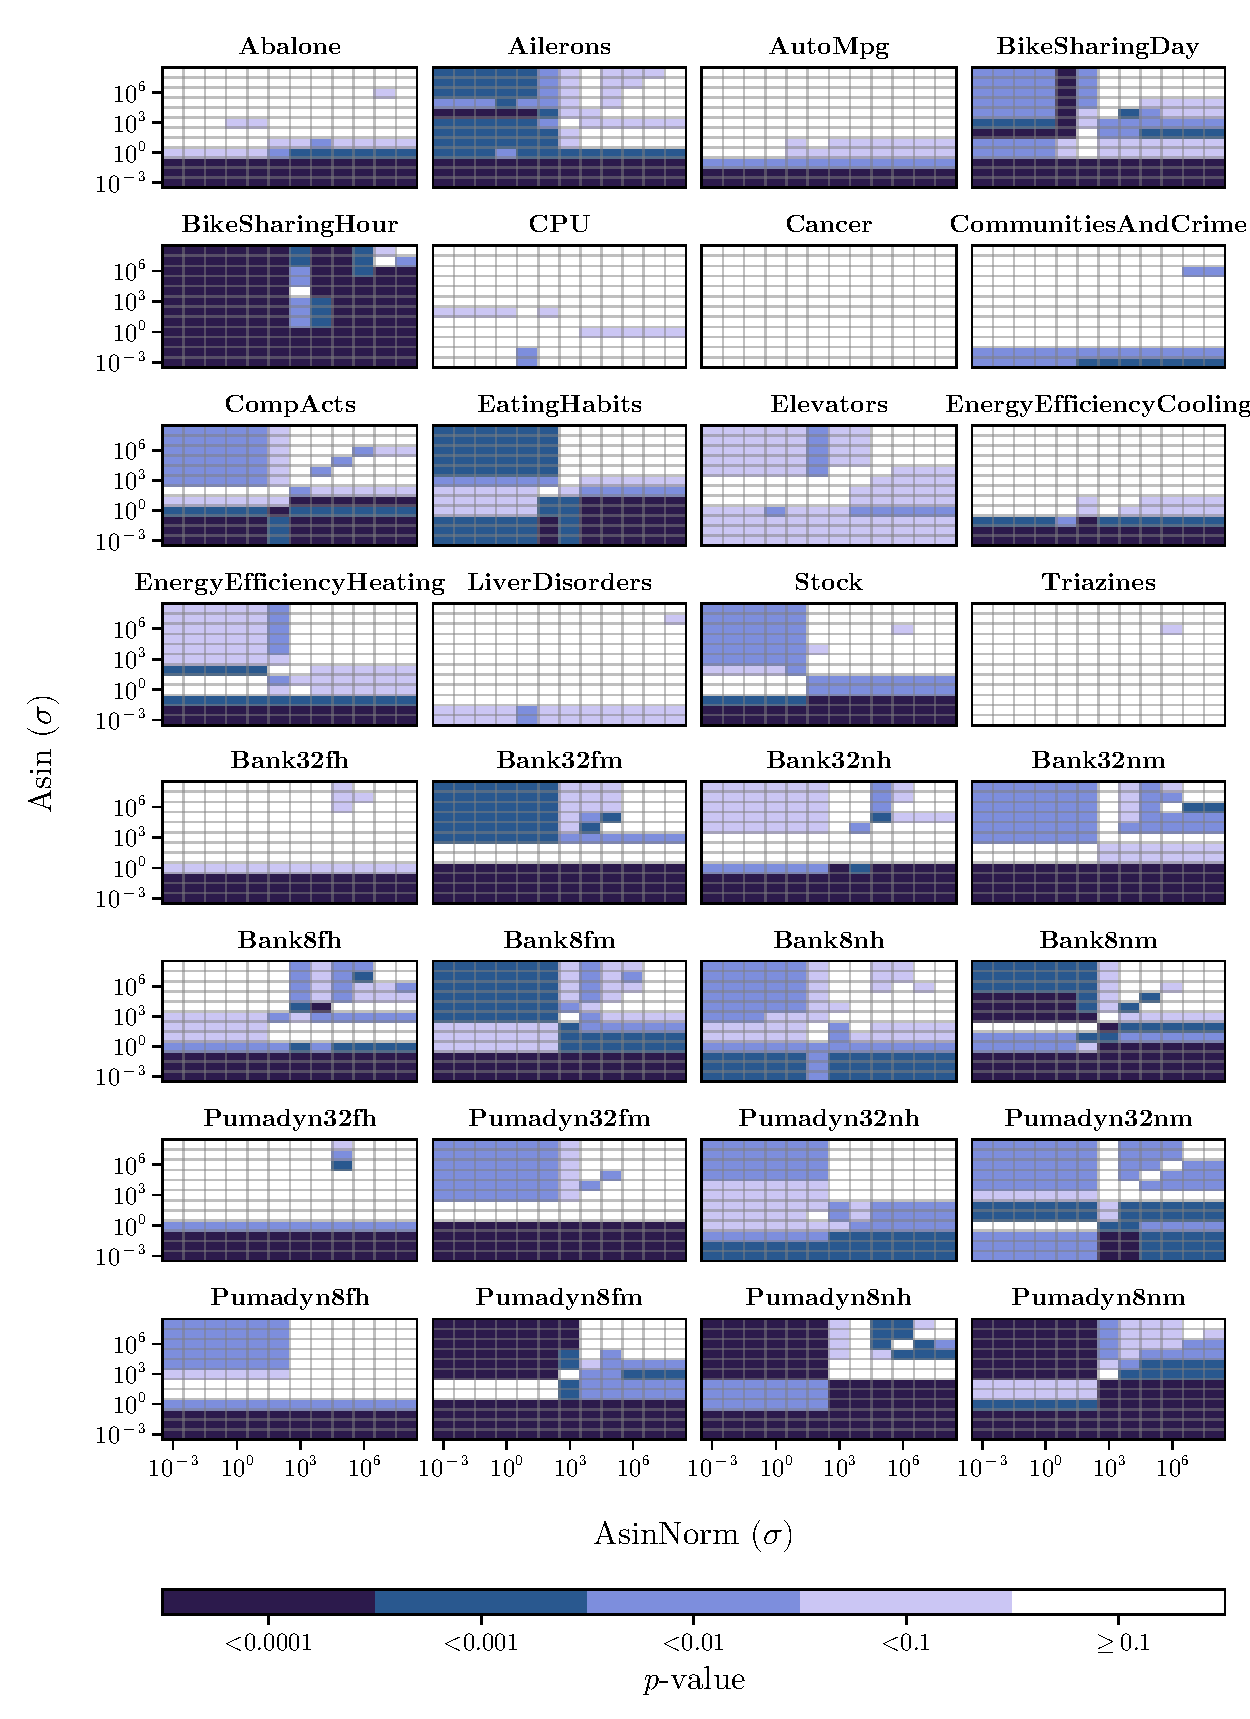
\includegraphics[width=0.9\textwidth]{plots/heatmaps_asin_asinnorm_pvalues}
    \caption{Difference between nRMSE of arc-sine and normalized arc-sine kernels}
    \label{fig:heatmaps-asin-asinnorm}
\end{figure}

\section{Training costs and drawbacks}

All the analysis done so far has been based on the $nRMSE$ performance measure
considering the best values of $\epsilon$ and $C$ for each dataset. However,
the training cost of the SVM is also an important factor to consider.

Indeed, we can conclude that under certain conditions, the rbf and arc-sine
kernels perform similarly, but does the training time also match?

While running the experiments, we measured both the training time and the
number of iterations needed to train the SVM. These give more information
about the cost of training the SVM than the $nRMSE$ alone.

\begin{cnote}
    Below are some RAW plots of the training time and number of iterations
    from the best models of each kernel and dataset combination.
\end{cnote}
\begin{figure}[H]
    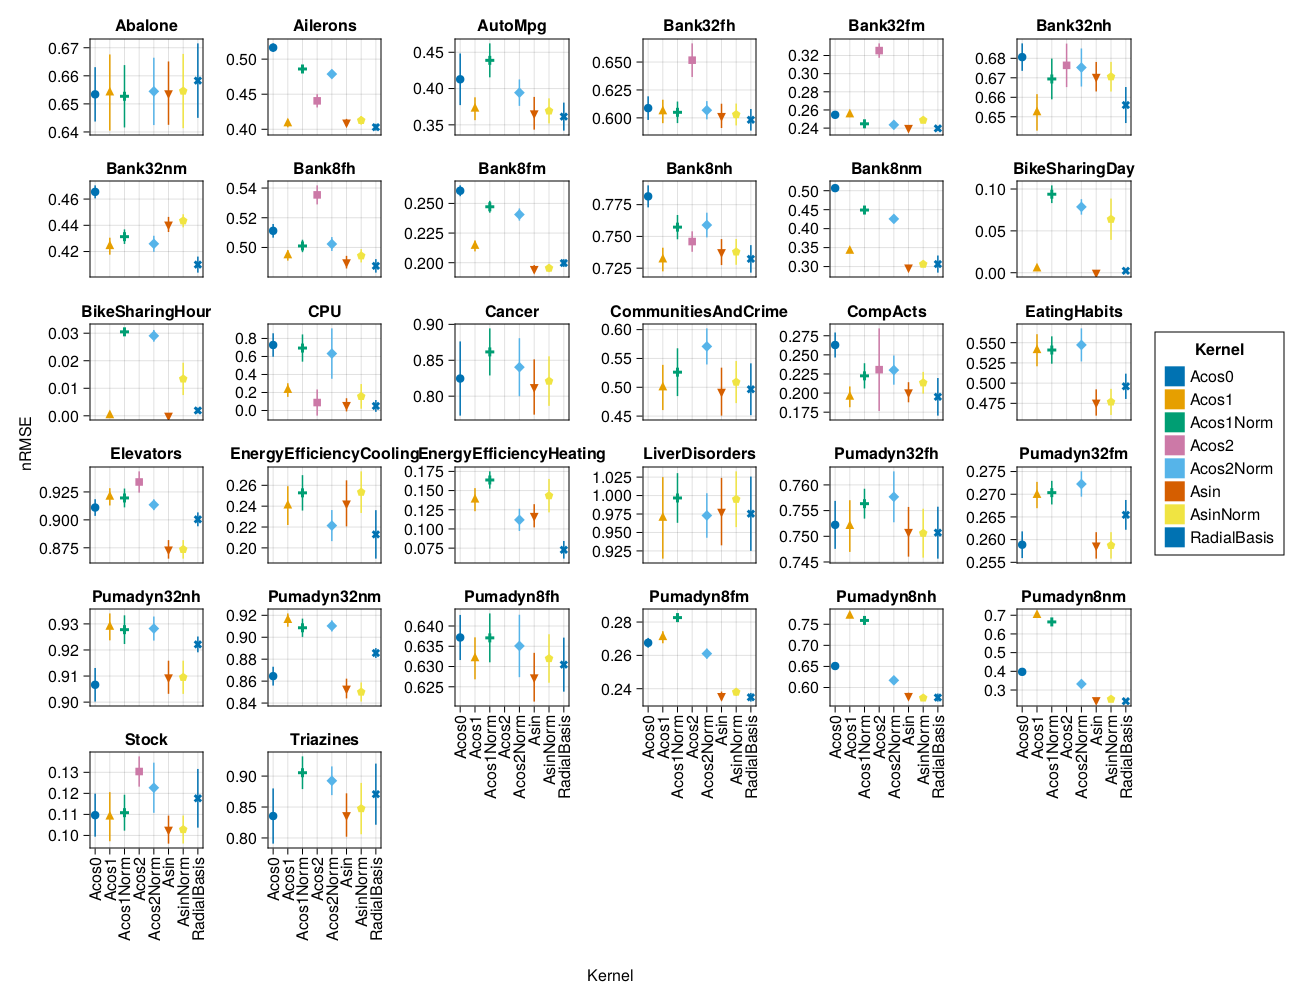
\includegraphics{raw_kernel_rmse_best}
    \caption{Best $nRMSE$}
\end{figure}
\begin{figure}[H]
    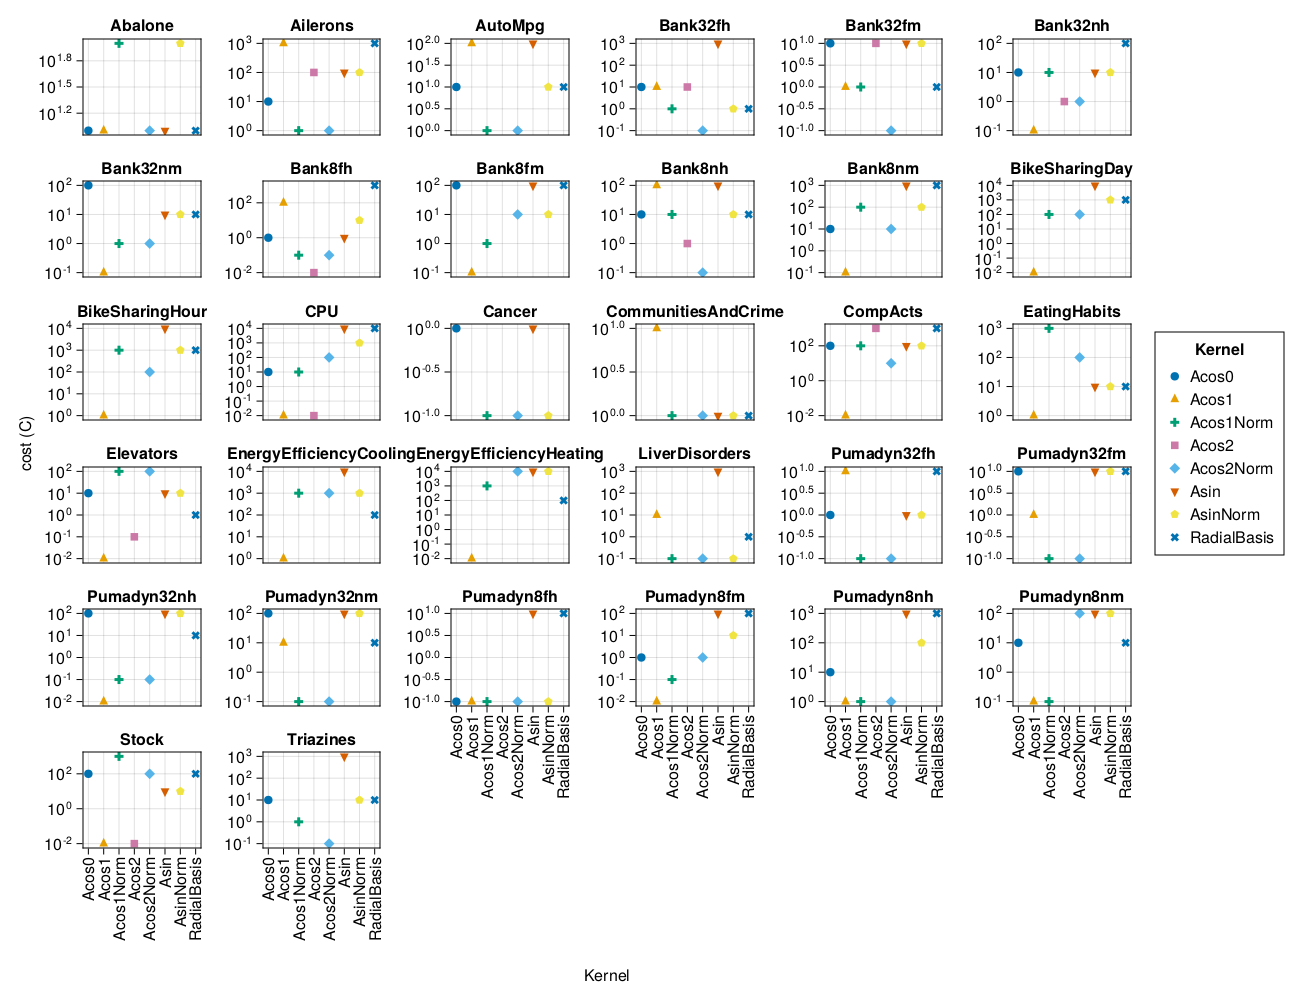
\includegraphics{raw_kernel_cost_best}
    \caption{Best $nRMSE$ Cost parameter}
\end{figure}
\begin{figure}[H]
    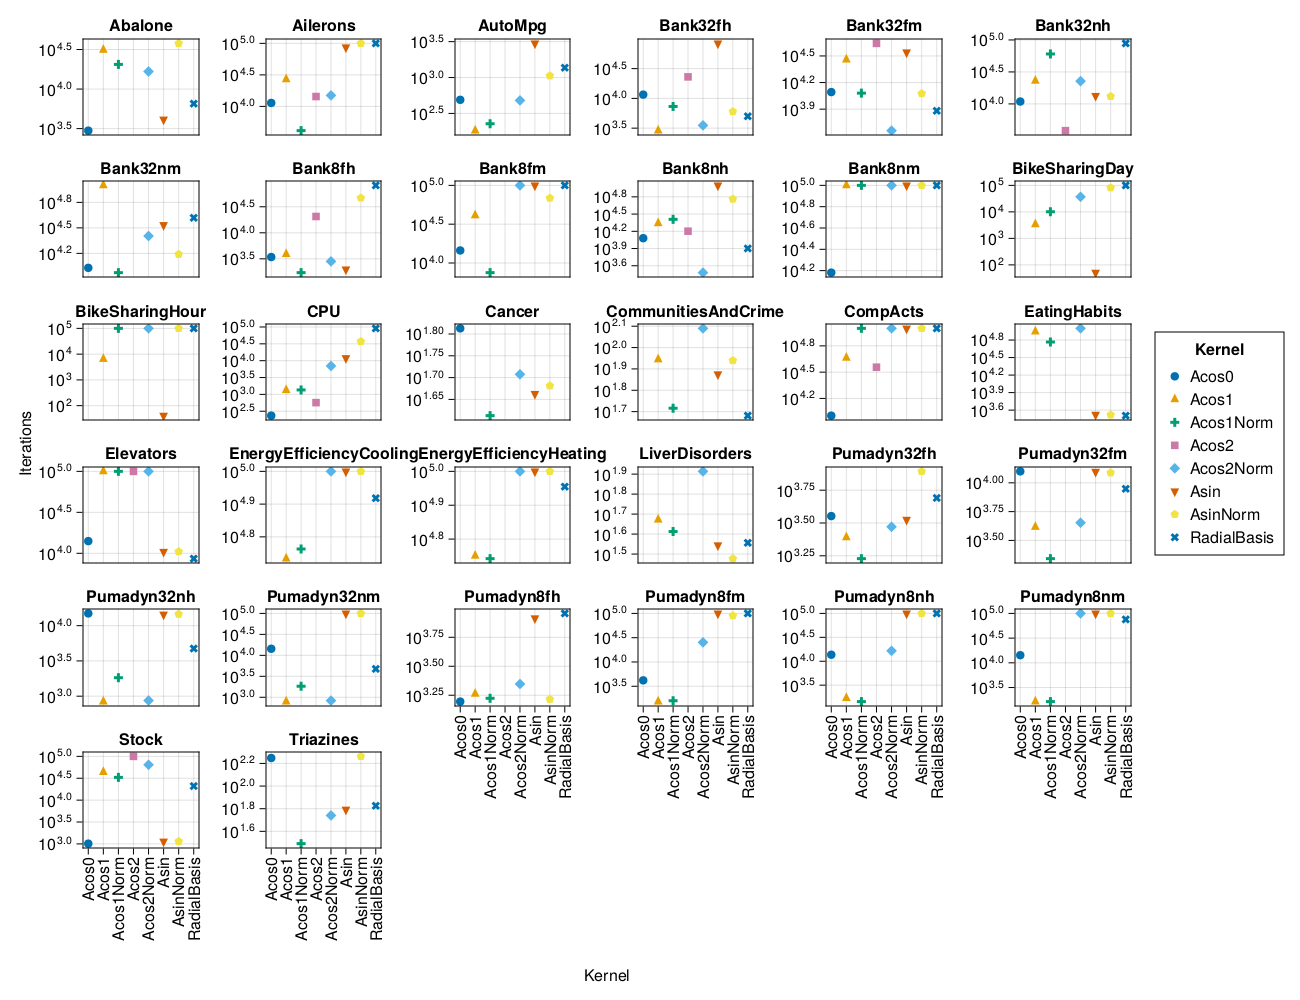
\includegraphics{raw_kernel_iterations_best}
    \caption{Number of iterations for the best models}
\end{figure}
\begin{figure}[H]
    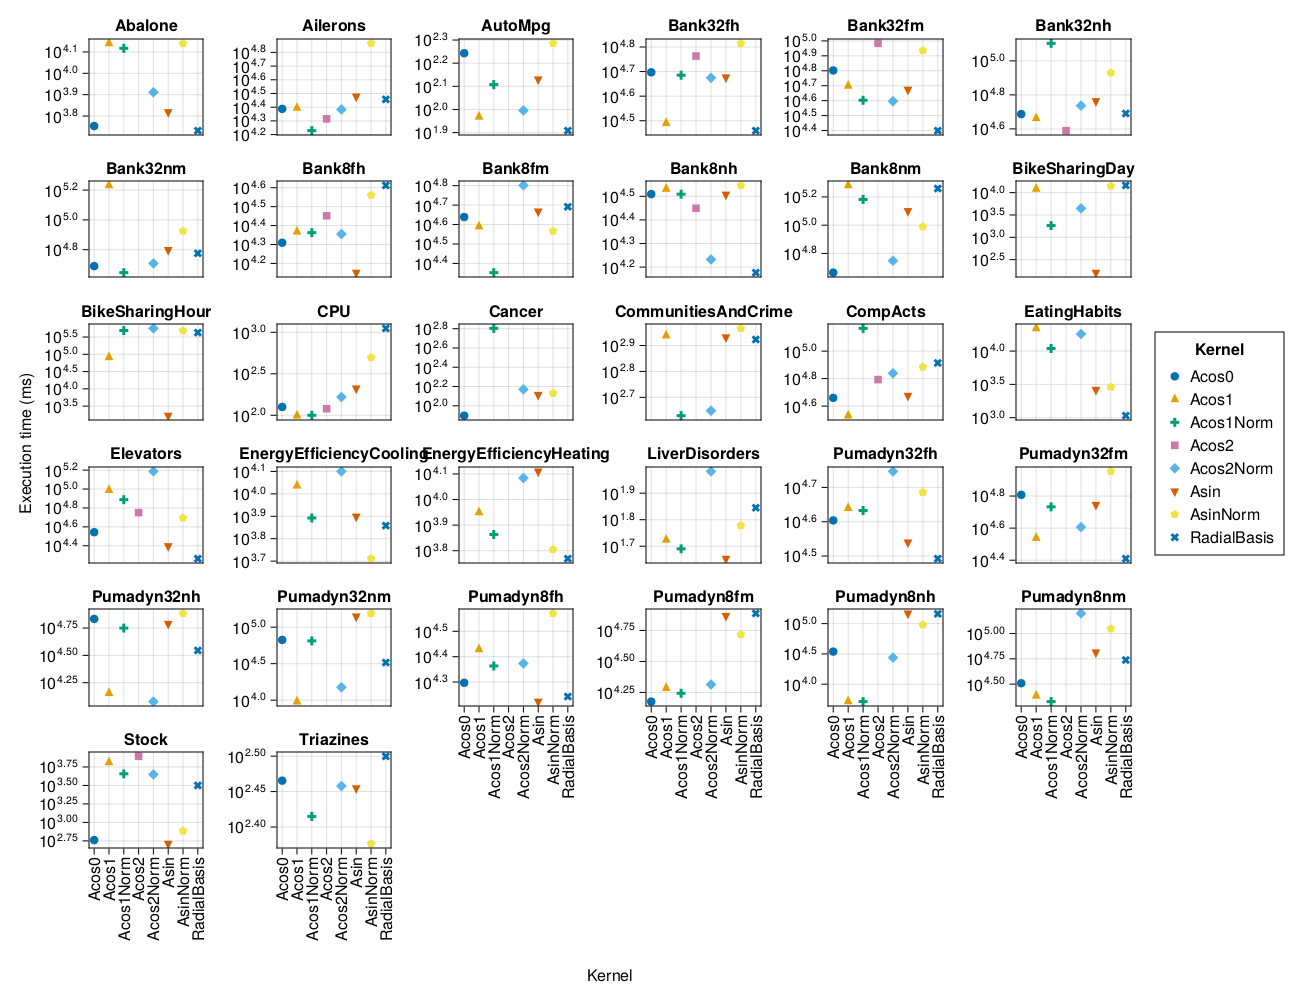
\includegraphics{raw_kernel_time_best}
    \caption{Training time for the best models}
\end{figure}

% TODO: maybe a combination plot of the heatmap and the line plot for some
% interesting datasets?

% TODO: classification is a mess
% \section{Classification}
%
% \begin{figure}[H]
%     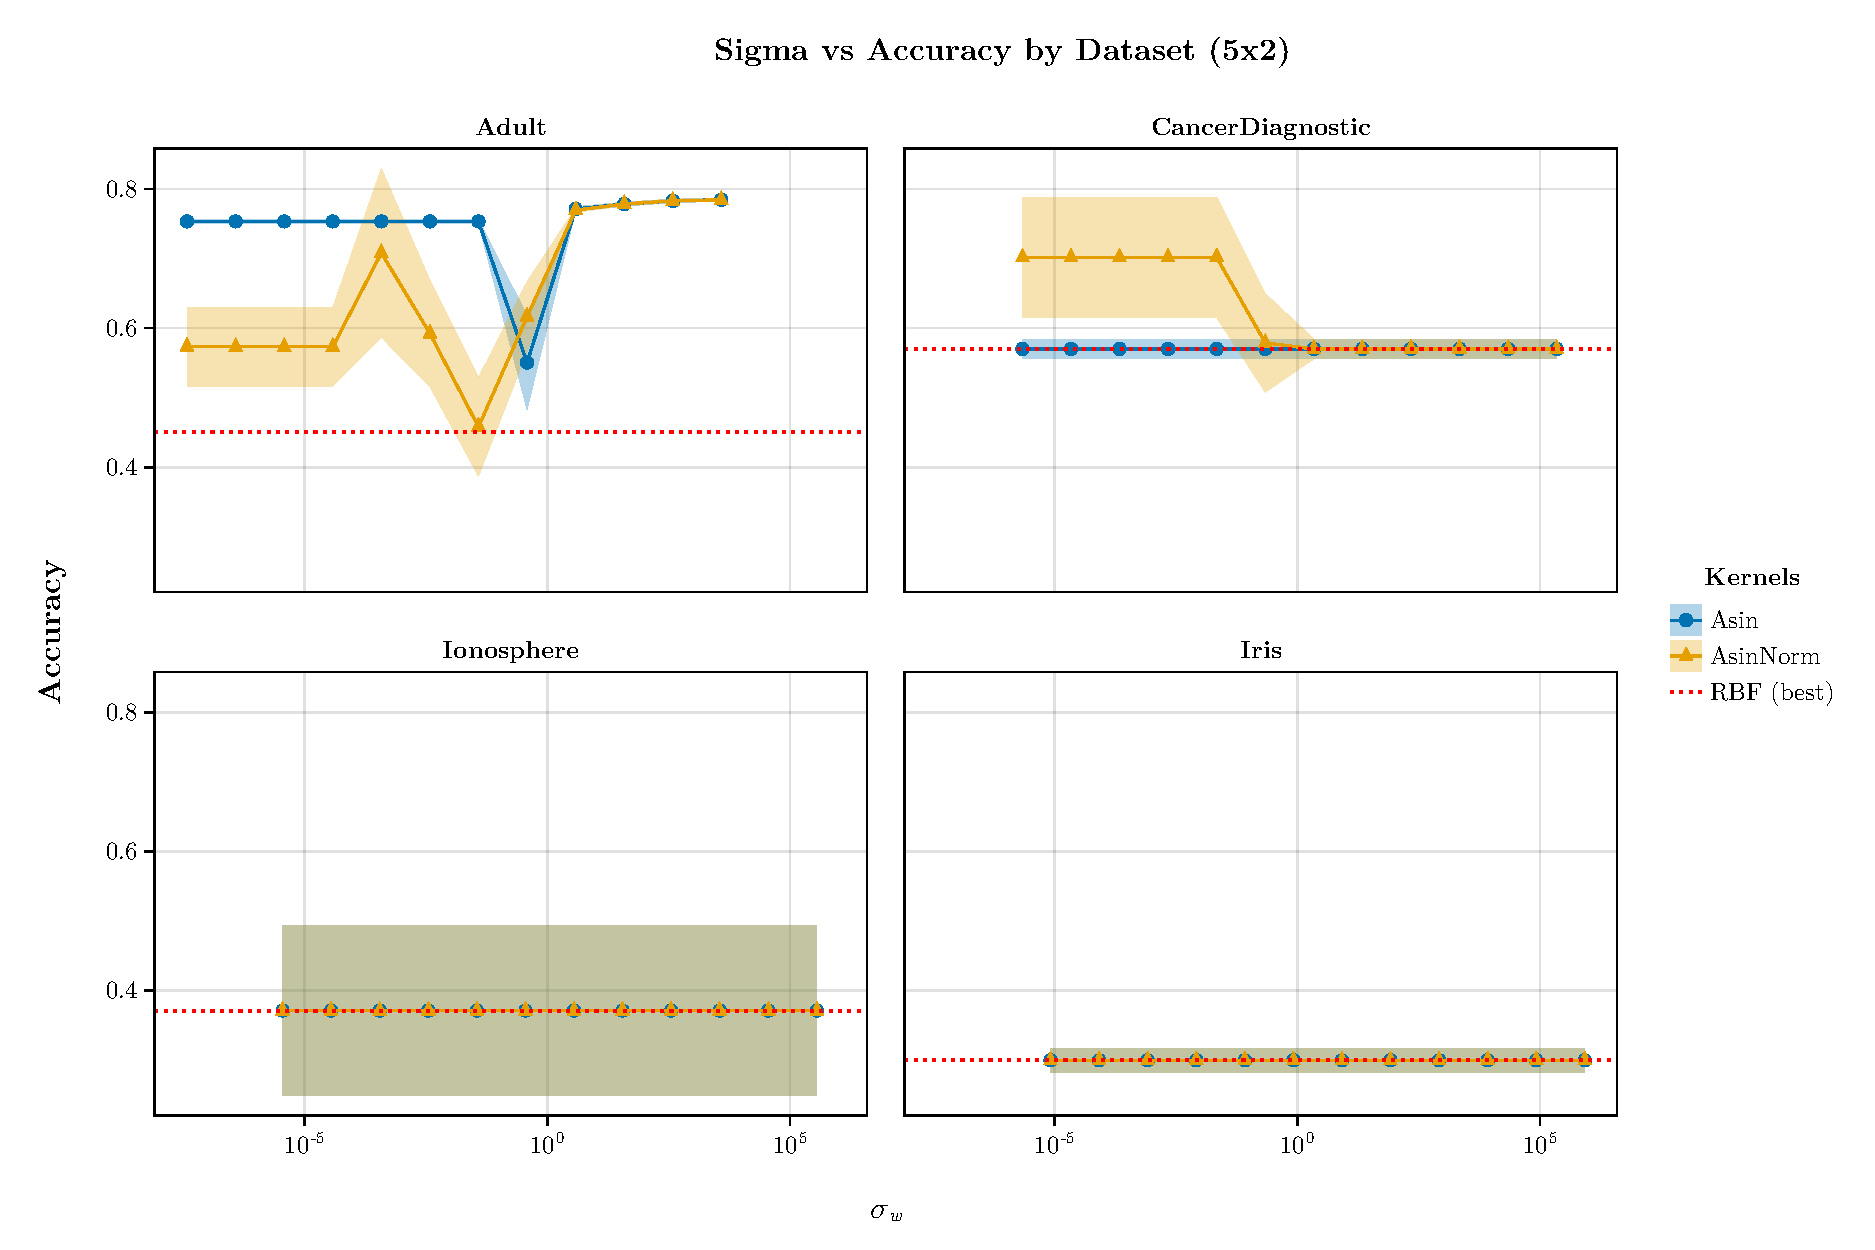
\includegraphics{plots/nRMSE_class_all_scaled}
%     \caption{Classification accuracy}
%     \label{fig:nrmse-class-all}
% \end{figure}
%
% \begin{marker}
%     This makes no sense, the accuracies are too low, specially iris (Even on the
%     RBF).
%
%     Add the other datasets.
%     Add more values of sigma.
%     Other metrics (precision, recall, f1, etc)
% \end{marker}

% \section{Estimation of the time needed to train the SVM}
%
% The main incentive for using the arc-sine kernel is that it is supposed to be
% parameter insensitive, which means that we can reduce the search space for the
% hyperparameters and thus reduce the time needed to train the SVM.
%
% If for the RBF kernel we have to search for $n$ possible values of $\gamma$
% hyperparameter whilst for the arc-sine kernel we can set $\sigma_w=10$ and
% achieve similar results, then we can reduce the search space by a factor of $n$.
%
% However, it is still possible that even with a fixed $\sigma_w$ the arc-sine
% kernel requires a wider search space for the other hyperparameters (cost and
% $\varepsilon$) or the computation of the kernel is more expensive than the RBF
% and thus the time needed to train the SVM is not reduced.
%
% For instance, in the initial testing of the normalized arc-sine kernel, the average
% training for the Adult dataset using the normalized arc-sine kernel
% took approximately 2 times longer than the RBF kernel.

% TODO: plots de temps de execucio
% TODO: plots de temps de iteracions / iteracions per segon
% TODO: plots de temps de nombre de parametres provats
%

\section{Meta-learning}

As explained in \cref{sec:meta-learning}, we want to use meta-learning
techniques to determine the best value of sigma for a given dataset, or at least
to determine if a dataset is a good candidate for the arc-sine kernel or not.
For that, we can create two models:
\begin{enumerate}
    \item Predict the best value of $\sigma_w$ for a given dataset.
    \item Predict whether a high value of $\sigma_w$ will achieve equivalent
          performance to the RBF kernel.
\end{enumerate}

For the first model,
we can use the best value of $\sigma_w$ for each dataset
obtained from the previous experiments. This will be our target
variable.

For the second model, we need to determine if there is a statistically
significant difference between the performance at $\sigma \gg 10$ and the
performance of the RBF kernel.
% TODO: t-test or arbitrary threshold?

% TODO: probably need a lot more datasets to be able to do anything...

\begin{note}
    With the number of datasets the results are not conclusive.
    Need much more datasets.
\end{note}
